\documentclass[12pt]{article}

% Set page size and margins
\usepackage[letterpaper,top=2cm,bottom=2cm,left=3cm,right=3cm,marginparwidth=1.75cm]{geometry}

% Useful packages
\usepackage{graphicx}
\usepackage{amsmath}
\usepackage{float}

\title{AM 213A HW3}
\author{Joseph Moore}
\date{Winter 2022}

\newenvironment{amatrix}[1]{%
	\begin{array}{@{}*{#1}{c}|c@{}}
	}{%
	\end{array}
}

\begin{document}

\maketitle

\title{\textbf{Part 1}}
 
\paragraph{a)}
	\subparagraph{$\bullet$}
		The first ten singular values are as follows,
		\[\begin{matrix}
		\sigma_1 = 663180.202318 \\
		\sigma_2 = 85706.595735 \\
		\sigma_3 = 62129.025680 \\
		\sigma_4 = 34664.633004 \\
		\sigma_5 = 31861.792296 \\
		\sigma_6 = 21872.721620 \\
		\sigma_7 = 19628.442780 \\
		\sigma_8 = 18434.937653 \\
		\sigma_9 = 13693.815446 \\
		\sigma_{10} = 12815.208252.
		\end{matrix}	
		\]
		The $k^{th}$ singular values are as follows,
		\[\begin{matrix}
		\sigma_{20} = 7528.024652  \\
		\sigma_{40} = 5489.124664  \\
		\sigma_{80} = 3948.779979  \\
		\sigma_{160} = 2668.223578 \\
		\sigma_{320} = 1515.865932 \\
		\sigma_{640} = 821.893126  \\
		\sigma_{1280} = 513.568032 \\
		\sigma_{2560} = 179.115035 \\
		\end{matrix}	
		\]
		The very last singular value is $\sigma_{3355} = 16.724645$

\newpage	
	\subparagraph{$\bullet$}
		The matrix of singular values corresponds to the level of image compression depicted below.\\
	
		$\Sigma_{\sigma_{20}}$ creates the image \\
		\includegraphics[scale=0.8]{part1/prob_a/Figure_1} \\
		$\Sigma_{\sigma_{40}}$ creates the image \\
		\includegraphics[scale=0.8]{part1/prob_a/Figure_2} \\
\newpage
		$\Sigma_{\sigma_{80}}$ creates the image \\
		\includegraphics[scale=0.8]{part1/prob_a/Figure_3} \\
		$\Sigma_{\sigma_{160}}$ creates the image \\
		\includegraphics[scale=0.8]{part1/prob_a/Figure_4} \\
\newpage
		$\Sigma_{\sigma_{320}}$ creates the image \\
		\includegraphics[scale=0.8]{part1/prob_a/Figure_5} \\
		$\Sigma_{\sigma_{640}}$ creates the image \\
		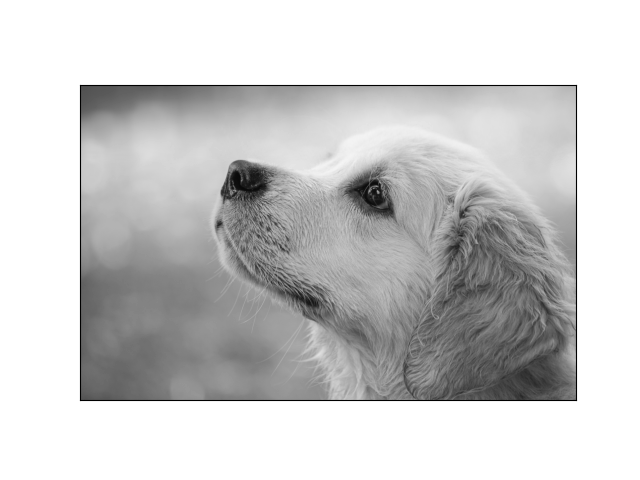
\includegraphics[scale=0.8]{part1/prob_a/Figure_6} \\
\newpage
		$\Sigma_{\sigma_{1280}}$ creates the image \\
		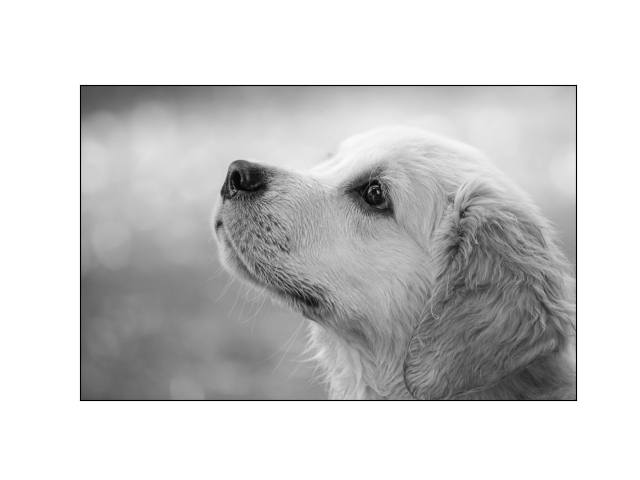
\includegraphics[scale=0.8]{part1/prob_a/Figure_7} \\
		$\Sigma_{\sigma_{2560}}$ creates the image \\
		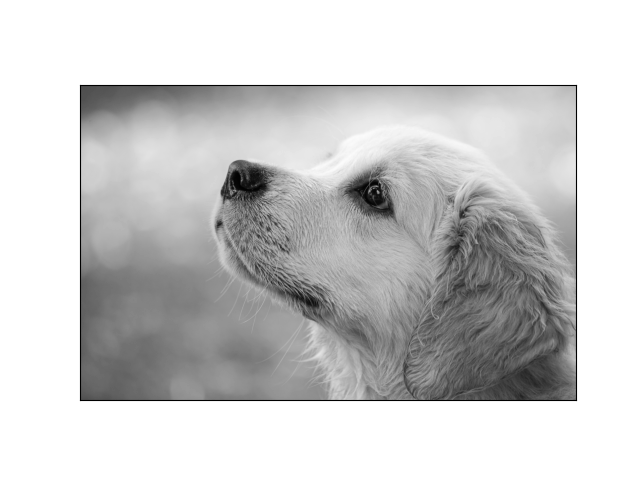
\includegraphics[scale=0.8]{part1/prob_a/Figure_8} \\
\newpage		
		$\Sigma_{\sigma_{3355}}$ is the all the singular values and thus is the original image \\
		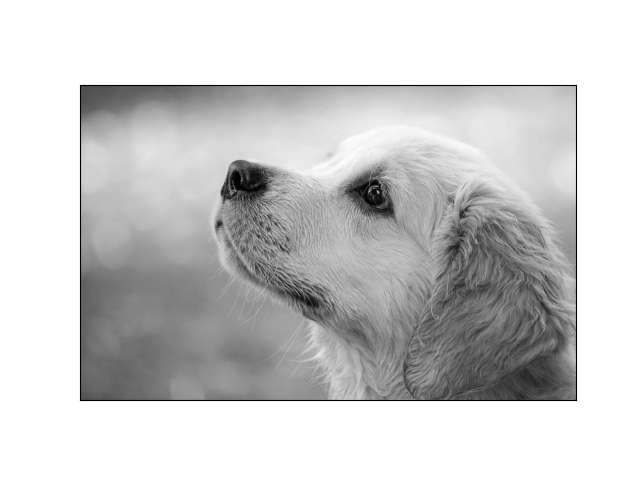
\includegraphics[scale=0.8]{part1/prob_a/Figure_9} \\

	\subparagraph{$\bullet$}	
		\[
		E_{20} = \frac{||A - A_{\sigma_{20}}||_F}{mn} = 0.003543
		\]\[
		E_{40} = \frac{||A - A_{\sigma_{40}}||_F}{mn} = 0.003166
		\]\[
		E_{80} = \frac{||A - A_{\sigma_{80}}||_F}{mn} = 0.002703
		\]\[
		E_{160} = \frac{||A - A_{\sigma_{160}}||_F}{mn} = 0.002156
		\]\[
		E_{320} = \frac{||A - A_{\sigma_{320}}||_F}{mn} = 0.001604
		\]\[
		E_{640} = \frac{||A - A_{\sigma_{640}}||_F}{mn} = 0.001173
		\]\[
		E_{1280} = \frac{||A - A_{\sigma_{1280}}||_F}{mn} = 0.000711
		\]\[
		E_{2560} = \frac{||A - A_{\sigma_{2560}}||_F}{mn} = 0.000187
		\]
		
		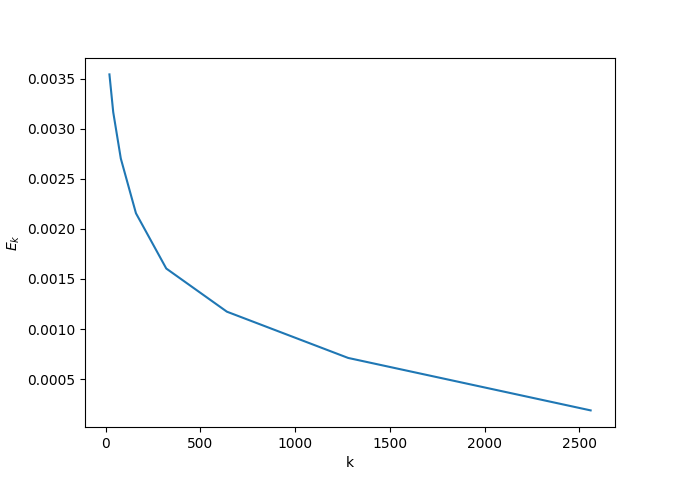
\includegraphics{part1/prob_a/Figure_10}
		
		As the number of singular values increases the image becomes closer to the original. The error falls like $\frac{1}{k}$ and appears to asymptotically approach zero. This tells us that we can get most of the information we need from the first few singular values. The higher we up k the less information is added to our image. At $k = 1280$ the error is below $10^{-3}$. However, from the graph we can tell that the error drops below $10^{-3}$ closer to $k = 1000$. With far less than half the total number of singular values we have a very small error.
	
\paragraph{b.1)}
	\subparagraph{$\bullet$}
		Both the Gauss-Jacobi and the Gauss-Seidel use an iterative method to solve $Ax = b$ for $x$. The Gauss-Jacobi simply splits up $A$ into its diagonal and remaining elements like $A = D + R$ and then follows $x^{k+1} = D^{-1}(b - Rx^k)$ until $x$ converges to a result. Gauss-Jacobi converges when $\rho(D^{-1}R) < 1$. Gauss-Jacobi further splits $R$ into upper and lower triangular matrices so that $A = L + D + U$. Gauss-Seidel follows $x^{k+1} = D^{-1}(b - Lx^{k+1} - Ux^{k})$ and converges for any symmetric, positive definite matrix. Gauss-Seidel converges faster than Gauss-Jacobi when they both converge. 
		
	\subparagraph{$\bullet$}
		The fist two plot for $D = 2$ and $D = 5$ have no Jacobi algorithm because it wouldn't converge.
		
		\includegraphics[scale=0.9]{part1/prob_b/Figure_1}
		
		\includegraphics[scale=0.9]{part1/prob_b/Figure_2}
		
		\includegraphics[scale=0.9]{part1/prob_b/Figure_3}
		
		\includegraphics[scale=0.9]{part1/prob_b/Figure_4}
		
		\includegraphics[scale=0.9]{part1/prob_b/Figure_5}
	
	\subparagraph{$\bullet$}
		The Jacobi algorithm did not converge on the first two runs likely because our matrix failed the test $\rho(D^{-1}R) < 1$. The Seidel algorithm converged for all of the runs as all the matrices were symmetric and positive definite. The Seidel algorithm also converged much faster each time both algorithms converged. The difference, however, seemed to close as the $D$ increased and Jacobi converged more easily.
		
	\subparagraph{$\bullet$}
		Setting $a_{ii} = i$ resulted in convergence for the Seidel algorithm but not for the Jacobi algorithm.
		
\paragraph{b.2)}
	\subparagraph{$\bullet$}
		The Conjugate Gradient algorithm for $Ax = b$ can be thought of as the following steepest decent on a quadratic equation. Because a quadratic equation only has one minimum then we are guaranteed to approach that minimum as long as we follow a decent direction. Because we are choosing the steepest decent, which must be orthogonal to all of the previous iterations decent directions, we must find the minimum in m iterations.
	
	\subparagraph{$\bullet$}
		First we acknowledge that all $r_i^Tr_j = 0$ for all $i \ne j$.
		\[
		p_0 = r_0 \Rightarrow p_0^Tr_0 = r_0^Tr_0
		\]\[
		p_1 = r_1 + \beta p_0 \Rightarrow p_1^Tr_1 = (r_1^T+\beta p_0^T)r_1 = r_1^Tr_1 + \beta p_0^Tr_1
		= r_1^Tr_1 + \beta r_0^Tr_1 = r_1^Tr_1
		\]\[
		p_2 = r_2 + \beta p_1 \Rightarrow p_2^Tr_2 = (r_2^T+\beta p_1^T)r_2 = r_2^Tr_2 + \beta p_1^Tr_2
		= r_2^Tr_2 + \beta r_1^Tr_2 = r_2^Tr_2
		\]
		Which continues like this showing that $p_k^Tr_k = r_k^Tr_k$. From this we see that $\alpha$ is the same. 
		\[
		E_{new} = r_k^Tr_k = p_k^Tr_k
		\]
		We now show that $\beta$ is the same for both. 
		\[ 
		r_{k+1} = r_k - \alpha Ap_k \Rightarrow Ap_k = r_k-r_{k+1}
		\]\[
		\beta = -\frac{r_{k+1}^Ty_k}{p_k^Ty_k} = -\frac{r_{k+1}^TAp_k}{p_k^TAp_k} =
		-\frac{r_{k+1}^T(r_k-r_{k+1})}{p_k^T(r_k-r_{k+1})} = \frac{r_{k+1}^Tr_{k+1}}{p_k^Tr_k} 
		= \frac{r_{k+1}^Tr_{k+1}}{r_k^Tr_k} = \frac{E_{new}}{E}
		\]
		From all this it becomes trivial to show that the two algorithms are equivalent. 
	
	\subparagraph{$\bullet$}
		It's clear that the Conjugate Gradient algorithm not only requires more iterations but also gets worse as the D increases. This, however, is not the same as computational time. It might very well be that CG has much faster iterations. Below is a table showing the number of iterations for each algorithm and D value.
		
		\begin{table}[H]
			\begin{tabular}{|l|l|l|l|l|l|}
				\hline
				& D = 2 & D = 5 & D = 10 & D = 100 & D = 1000 \\ \hline
				Jacobi & \begin{tabular}[c]{@{}l@{}}Does not \\ converge\end{tabular} & \begin{tabular}[c]{@{}l@{}}Does not \\ converge\end{tabular} & 137 & 6 & 4 \\ \hline
				Seidel & 59 & 17 & 10 & 4 & 3 \\ \hline
				\begin{tabular}[c]{@{}l@{}}Conjugate \\ Gradient\end{tabular} & 1109 & 1707 & 3559 & 190429  & 19712896 \\ \hline
			\end{tabular}
		\end{table}
	
	\subparagraph{$\bullet$}
		We can show that the eigenvalues of our matrix are $D-1$ and $D+9$ where $D$ is the value of the diagonal elements. This means that the matrix is already relatively well conditioned.
	
	\subparagraph{$\bullet$}	
		For the 10x10 matrix where $a_{ii} = i$ CG converges in 4474 iterations. The 100x100 diverges immediately. In fact, from testing I find that anything over 12 diverges immediately.
	
	
\end{document}